\documentclass{sigchi}

% Remove or comment out these two lines for final version
\toappearbox{\Large Submitted to CHI'13. \\Do not cite, do not circulate.}
\pagenumbering{arabic}% Arabic page numbers for submission. 

% Use \toappear{...} to override the default ACM copyright statement (e.g. for preprints).

% Load basic packages
\usepackage{balance}  % to better equalize the last page
\usepackage{graphicx} % for EPS, load graphicx instead
\usepackage{times}    % comment if you want LaTeX's default font
\usepackage{url}      % llt: nicely formatted URLs
\usepackage{tabularx}
\usepackage{subfigure}

% llt: Define a global style for URLs, rather that the default one
\makeatletter
\def\url@leostyle{%
  \@ifundefined{selectfont}{\def\UrlFont{\sf}}{\def\UrlFont{\small\bf\ttfamily}}}
\makeatother
\urlstyle{leo}


% To make various LaTeX processors do the right thing with page size.
\def\pprw{8.5in}
\def\pprh{11in}
\special{papersize=\pprw,\pprh}
\setlength{\paperwidth}{\pprw}
\setlength{\paperheight}{\pprh}
\setlength{\pdfpagewidth}{\pprw}
\setlength{\pdfpageheight}{\pprh}

% Make sure hyperref comes last of your loaded packages, 
% to give it a fighting chance of not being over-written, 
% since its job is to redefine many LaTeX commands.
\usepackage[pdftex]{hyperref}
\hypersetup{
pdftitle={SIGCHI Conference Proceedings Format},
pdfauthor={LaTeX},
pdfkeywords={SIGCHI, proceedings, archival format},
bookmarksnumbered,
pdfstartview={FitH},
colorlinks,
citecolor=black,
filecolor=black,
linkcolor=black,
urlcolor=black,
breaklinks=true,
}

% create a shortcut to typeset table headings
\newcommand\tabhead[1]{\small\textbf{#1}}


% End of preamble. Here it comes the document.
\begin{document}

\title{Making Touchscreen Keyboards Adaptive to Keys, Hand Postures,  and Individuals - A Hierarchical Spatial Backoff Model Approach}

% Note that submissions are blind, so author information should be omitted
\numberofauthors{3}
\author{
  \alignauthor 1st Author Name\\
    \affaddr{Affiliation}\\
    \affaddr{Address}\\
    \email{e-mail address}\\
  \alignauthor 2nd Author Name\\
    \affaddr{Affiliation}\\
    \affaddr{Address}\\
    \email{e-mail address}\\
  \alignauthor 3rd Author Name\\
    \affaddr{Affiliation}\\
    \affaddr{Address}\\
    \email{e-mail address}\\
}

% Teaser figure can go here
%\teaser{
%  \centering
%  \includegraphics{Figure1}
%  \caption{Teaser Image}
%  \label{fig:teaser}
%}

\maketitle

\begin{abstract}
The underlying spatial model of a touchscreen keyboard can adapt to factors such as input hand postures, individuals, and target key positions to improve the text entry prediction on mobile devices. To 
combine these factors together, we introduce a hierarchical spatial backoff
model (SBM) that consists of submodels with different levels of
complexity. The most specific model adapts to 
all three factors whereas the most general model is independent
of all these adaptive factors. Considering that in practical use people may switch hand postures (e.g., from two-thumb to one finger) to suit a situation and the specific submodels may take time to train for each user,  a specific submodel is applied only if its corresponding input posture is identified with confidence and if the submodel has enough training data from the user.  We introduce
the \textit{backoff} mechanism to fall back to a simpler model if either of these conditions are not met. Overall the SBM with the most specific model (posture, individual, and key adaptive) gives a 13.2\% reduction in character error rate compared to the base model. We also
developed an online input posture classification method for touchscreen keyboard which can be
used with the adaptive spatial model to improve the key estimation accuracy.
 
\end{abstract}

\keywords{
  Touchscreen text input; posture adaptation; personalization; adaptive model.
}

\category{H.5.2.}{Information interfaces and presentation}{User interfaces -- \textit{input devices and strategies}}

\section{Introduction}
The rapid growth of touchscreen based smartphones and tablets have made finger typing on touchscreens an everyday information input activity. Touchscreen keyboards, which can also be called Smart Touch Keyboards (STK’s) have advanced significantly in the past few years. Taking the publicly available open source Android keyboard as an example, a modern touch screen keyboard uses language modelling, spatial and edit distance based corrections, and other sophisticated techniques to predict, correct, and complete the user’s imprecise typing. Despite these engineering achievements, text input continues to be a mobile user experience bottleneck, particularly for business and productive use~\cite{Bao:2011}. Any further improvement to the mobile typing experience, even by a small amount, is desired and important considering hundreds of millions of people use their smartphone or tablet everyday.

One compelling direction of research is better adaptation and personalization of keyboard spatial models. A spatial model converts each touch point into a probability distribution over the different letters on the keyboard. With soft keyboards, the underlying “keys” can shift and adapt to the individual user. Azednkot and Zhai~\cite{Azenkot:2012} did a systematic study of smartphone keyboard touch patterns under various typing conditions. We note the following observations based on their study:

\begin{enumerate}
\item People use different “hand postures” -- one finger, one thumb, and two thumbs -- to type on smartphones. Depending on the situation (e.g. sitting, standing or walking), the same individual may also change from one hand posture to another. For example, the same individual who normally types with two thumbs on a phone while sitting down may switch to one finger or one thumb typing while standing or walking. We cannot assume that the same individual will use the same hand posture all the time. Adaptation methods based on lab experiments with one consistent hand  posture, such as those in~\cite{Findlater:2012}, give important insights and guidance for designing practical systems. But they may also face challenges as practical solutions because user may change their hand posture in real world settings from their normal preference.

\item These hand postures change the touch typing patterns. For example for right handed users one finger and one thumb typing on the left side of a smartphone touchscreen keyboard tend to biased towards to the right direction, whereas two thumb typing on the left side of the keyboard tend to shift to the left direction.

\item Touch patterns can also be dependent on letter keys. For example for one finger typing users touch points tend to shift downward on the bottom letter row of a touchscreen keyboard, but not the top row. 

\item Users’ touch points tend to spread wider on a collective basis (polling all users data together) than on an individual basis. This shows that different users tend to have different touch point distributions, but within the same user, the touch point pattern using the same posture may be more consistent.
\end{enumerate}

Together these findings make a strong case for personalization of smartphone touch keyboard algorithms. However they also illustrate the challenges and complexities of personalization. An advanced keyboard that adapts to individual user differences needs to account for multiple \textit{adaptive factors} in order to work effectively. For example, a personalized typing model would have a major limitation if it does not also adapt to hand posture. This is because the same user can have a very different typing pattern depending on whether she is typing with one finger or two. Effective adaptation may require a combinatorial approach that is key, posture, and user specific. 

A combinatorial approach raises challenging implementation issues. First, there need to be a large number (e.g., 26 keys $\times$ 3 postures = 78) of submodels for each individual user. Collecting a sufficient amount of data to build each submodel may take too long to be practically useful, especially for infrequent letters such as Z and X. Second, if an STK does have a large number of (sub)models, model selection can be a significant challenge.  Since each submodel is specific to a combination of factors, a wrong selection may actually hurt the keyboard’s quality. Correct model selection requires an accurate identification of the current \textit{mode}, i.e. a combination of adaptive factors. While it is relatively easy to identify the individual (by for example device login) and letter key, it is not so easy to identify what hand posture the user is applying to each tap. 

To address these challenges, we propose and explore a hierarchical backoff approach to building adaptive STK spatial models. The models in the hierarchy range from generic (e.g. a base model that is user, key, and posture invariant) to specific (e.g. a model that has specialized parameters for each user, key, and posture combination). When a user first starts typing on an hierarchical adaptive keyboard, it initially defaults to the base model while other more specific models are dormant. Each touch input point from the user contributes to building the submodel(s) that the touch point belongs to (e.g., the user specific model for a particular key). When a submodel \textit{matures}, i.e. a sufficient amount of data is available to train it, it becomes active. Determining the threshold for the minimum amount of data required is an essential part of the backoff model and we will discuss our findings later in the paper.
A \textit{mature} model will continue to renew itself with new user data to accommodate  both short and long term adaptation to changes in user behavior. When multiple submodels are active the system chooses the highest level (most specific) model that has is both \textit{mature} and has a sufficiently high confidence (e.g., posture classification confidence). If either of these conditions is not met, meaning there is not enough data to train the model or the system is not confident enough that the model is appropriate, the system \textit{backs-off} to a more general model or the base model. This hierarchical backoff approach is a major contribution of this paper, and offers the following advantages for fast and robust adaptation in a STK:
\begin{enumerate}
\item It does combinatorial and fine grained adaptation, not only to the individual user as a single lumped entity, but also in combination with hand posture and key location factors. It is therefore more practical and less brittle since it does not assume one user would always use the same hand posture in all situations.

\item It is conservative. Posture adaptation is applied only if the posture detection is confident enough,, and when its corresponding submodel is \textit{mature}. It is also designed to be conservative and biases towards the standard base model if either of these condition is not clearly satisfied. This minimizes the risk of over adaptation and transitional instability when the user changes hand posture. 
 
\item The system does not require a separate training (data collection) phase for each individual. It is more practical to launch such an adaptive system.

\item The system continually updates and renewal itself, so it can accommodate long term changes in user behavior. 
\end{enumerate}
We call keyboards built in such an approach SBM (spatial backoff model) keyboards. The SBM approach also raises many questions and challenges which will be addressed in the rest of the paper. Here we give a brief outline to these problems and their solutions.

First, while the observations made in~\cite{Azenkot:2012} is quite unambiguous about key location, hand posture, and individual being reasonable adaptive factors, they need further investigation.  We report one analysis on the relative key detection power of various spatial models specific to the combinatorial factors of key, hand posture,  and individual in section ``Comparison of Spatial Model''. The analysis is based on \textit{observed} posture and user intended key. With our dataset it was found that posture and key specific spatial models could reduce character error rate by about 12.0\% compared to the key specific model only; and user and key specific spatial models could reduce character error rate by about 14.7\% compared to the key specific model. These reduction in error rates represent theoretical upper bounds based on our dataset. 

Second, in section ``Input Hand Posture Classification'' we present a detailed SVM-based classifier of hand postures that returns mode identification of two-thumb or one-finger (including one-thumb) posture from users' touch points while entering text.

Third, using the posture classification method and user adaptation, does higher order specific models really offer better error corrections than a lower order or base model without language model (as a baseline)? We address this question in the ``Evaluation of Standalone SBM'' section. With \textit{inferred} posture and user intended key, the posture, individual and key adaptive spatial model could reduce the character error rate by about 13.2\% compared to the base model which is key, posture and user invariant.

\section{Research Methods}
As smartphone keyboard become more sophisticated, and given the relatively complex solutions proposed that involve multiple components, multiple phases, and learning,  we fear the traditional lab experiments based HCI evaluation method may not be efficient or sensitive enough for researchers to make rapid progress. In this paper we use a combination of HCI and ML (machine learning) evaluation methods, along with algorithm and system development. 

We first select a smartphone typing dataset as the empirical basis of training and cross-validation. The experiment that generated the dataset had been peer reviewed and published. Briefly, the experiment involved 32 participants who were given random phrases to type on a “data collector” keyboard run on an Android touchscreen phone.  The participants were encouraged to type as naturally as possible and not to correct any errors. The goal was to collect user’s touch patterns by their natural instinct with little concern to technology constraint. The experiment was between-subject in which each participant used one hand posture to type. For consistency, we removed the data from 2 left-handed users in our analysis, and are left with data from 9 users using one-index-finger input, 11 users using one-thumb input and
10 users using two-thumb input.  Since we found much less difference between the index finger condition and the single thumb condition and due to posture classification reliability concerns, we combine index-finger and one-thumb input as one-finger input condition. Hence the posture class random variable $y$ can take values in the set $\mathcal{Y} = \{\text{one-finger}, \text{two-thumb}\}$. We also filtered out touch points that are 1.5 times the height of the key away from the center of the target key. After this, there are 84292 total touch points. For all evaluations, the ratio of the number of users using one-finger input to that using two-thumb input is kept the same for the training and testing datasets. 

A basic dependent variable (measure) of the dataset and any models built from it is “character error rate”. This is measured by the difference between the character in the target phrase and character determined from the touch point via a spatial model. Note although this rate can be viewed as a percentage of the total number of characters in the target phrase, it is to be interpreted with precaution. First, 0\% error rate may never be achievable given how the dataset was achieved. Second the absolute error rate maybe dataset dependent and is not necessarily what a user would experience in practice, but the comparative error rates across conditions are informative of the qualities of different models.

\section{Related Work}

There is a body of active research on using spatial model, language model, or a combination
of the two to improve text entry accuracy on a STK. For examples, 
Al Faraj et al. \cite{AlFaraj:2009} and Magnien et al. \cite{Magnien:2004} both use
visual highlight of the next possible keys to aid users' typing. Their predictions of the next keys are based on a language model. As our focus is on the 
spatial model, we also mainly look at the related work in this aspect.    

Kristensson et al. \cite{Kristensson:2005} propose a geometric pattern matching technique to improve 
stylus input accuracy. They match the geometric pattern of the touch points on a stylus keyboard against patterns formed by 
the letter key center positions of legitimate words in a lexicon. Similar to this approach,
they developed a gesture-based stylus input method where users only need to stroke between the keys \cite{Kristensson:2004}.
Their approaches essentially use a combination of spatial and language models. However, 
their spatial model is not adaptive. While our focus is on tapping input, the same adaptive spatial model approach
can be potentially applied to the gesture-based input.

In terms of spatial model that is adaptive to keys, Goodman et al. \cite{Goodman:2002} use bivariate Gaussian distribution with means, and
covariance matrices computed separately for each key in their study on stylus input. Zhai et al. \cite{Zhai:2002} also show that
the hit points for each key on a Metropolis keyboard \cite{Zhai:2000} are normally distributed and 
the centers of the distributions shift in different directions depending on the positions of
the keys. In their relative keyboard input system, Rashid et al. \cite{Rashid:2008} use a different bivariate Gaussian for each key. The error rate of their system is high because the lack of 
a priori determined keyboard position.

Building on \cite{Goodman:2002}, Gunawardana et al. \cite{Gunawardana:2010} use restricted bivariate Gaussian
models in their anchored key-target resizing method. Key-target resizing means dynamically
adjusting the underlying target areas of the keys based on their probabilities. The probabilities can 
be a combination of spatial model and language model probabilities.
They argue that overly aggressive
key-target resizing can sometimes prevent users from entering their desired text, and hence violate
users' expectation about keyboard functionality. They ensure that touch points within
the anchor area of a key is always detected as that key irrespective to the language model.

There is also a number of research related to personal adaptation. Findlater and Wobbrock~\cite{Findlater:2012} explored spatial model adaptation on large touch surfaces, where one can use ten fingers to do traditional desktop style touch typing. They find measurable performance improvements when the keyboard touch typing model is able to adapt to a particular user. This is quite plausible because users can have different typing styles, finger sizes, and hand shapes. They also find that changing the visual layout of the keyboard is not beneficial for ten-finger touch typing on large screens.

In comparison to ten-finger typing on a large touch surface, the individual differences in one-finger or two-thumb typing on smartphones are more subtle but still compelling. Rudchenko et al.~\cite{Rudchenko:2011}
developed a text entry game for smartphones that provides 
targeting words for users to type to improve their typing experience. As a side effect,
the game generates labeled touch point data which can be used as
training data to build the spatial models. They use the touch points from the first 10 rounds of each 
participant's game play to build the personalized model for each key, and simulate the key detection
process for the second 10 rounds. Their result shows that key-target resizing based on
spatial model only without personalization gives an error reduction of 18.9\% over no key-target resizing. When adding personalization, there is a further 2.84\% error reduction.
Their results show the benefit of individual adaptation in an ideal condition where the 
intended key is known. In the real world application, the keys users intend to hit are unknown and can only be inferred based on the current spatial and language models. In our prototype implementation and evaluation we impose the same real-world limitation. We build the user adaptive spatial model by probabilistically assigning a key to each of the user’s touch points, without relying on the hidden identity of the true intended key. 

The key and individual adaptive methods mentioned earlier all assume that users' input posture
remains the same. We observe that the same individual may change hand postures even on the same device. Building on the observations made in [1], we investigate how posture adaptation can be implemented and how it can actually affect key estimation accuracy.

The idea of backoff to a lower order model when a higher order more specific model is not available is commonly used in language modelling (LM) for speech recognition~\cite{Katz:1987, Zitouni:2007}. For example, when unseen \textit{n}-gram events are encountered, the backoff class based \textit{n}-gram language model is used.  In LM,  all context is observed including backoffs. However in our model some of the variables are observed, e.g. user, whereas some are hidden and need to be inferred, e.g. posture. As a result, the backoff conditions are more complicated in our model.

Finally, researchers have explored other dimensions to improve the 
text input experience on touchscreen keyboard. One dimension is using hardware
augmentations to provide vibro-tactile feedback \cite{Brewster:2007, Hoggan:2008}. 
Another dimension is using alternative keyboard layouts optimized for typing speed (wpm)
based on Fitts' law and character level digraph frequencies \cite{Zhai:2000, MacKenzie:1999}.
These dimensions are orthogonal to the language and the spatial models, and can be potentially 
combined together to further increase the input accuracy and speed.

\section{Hierarchical Spatial Backoff Models (SBM)}
The hierarchical adaptive SBM consists a number of submodels in different “orders” (Figure. \ref{fig:hierarchy}). Each submodel is represented by a bivariate Gaussian distribution~\cite{Azenkot:2012, Goodman:2002, Rashid:2008}.
The zeroth order is the base model which is key, individual, and posture
independent, i.e. all the keys have the same Gaussian distribution $N(\underline\mu, \Sigma)$
where $\underline\mu \in \mathbb{R}^2$ is the mean $(x, y)$ offsets from the center of
each key's bounding box, and $\Sigma$ is a $2\times 2$ covariance matrix. This is the most general model combining all data together. The
higher order submodels adapt to a combination of 
key positions, hand postures, and individuals. For example, the ``posture adaptive'' model, adapts to input posture only which means there is one Gaussian model $N(\underline\mu_y, \Sigma_y)$ for each posture $y$ for \textit{all} keys. The ``posture \& key adaptive'' model adapts to both posture and key which means there is one Gaussian model $N(\underline\mu_{y, k}, \Sigma_{y, k})$ for each posture $y$ and key $k$ combination.  The highest order model has one Gaussian model $N(\underline\mu_{y,u,k}, \Sigma_{y,u,k})$ for each posture $y$, user $u$ and key $k$ combination.

\begin{figure}[tb]
  \centering
  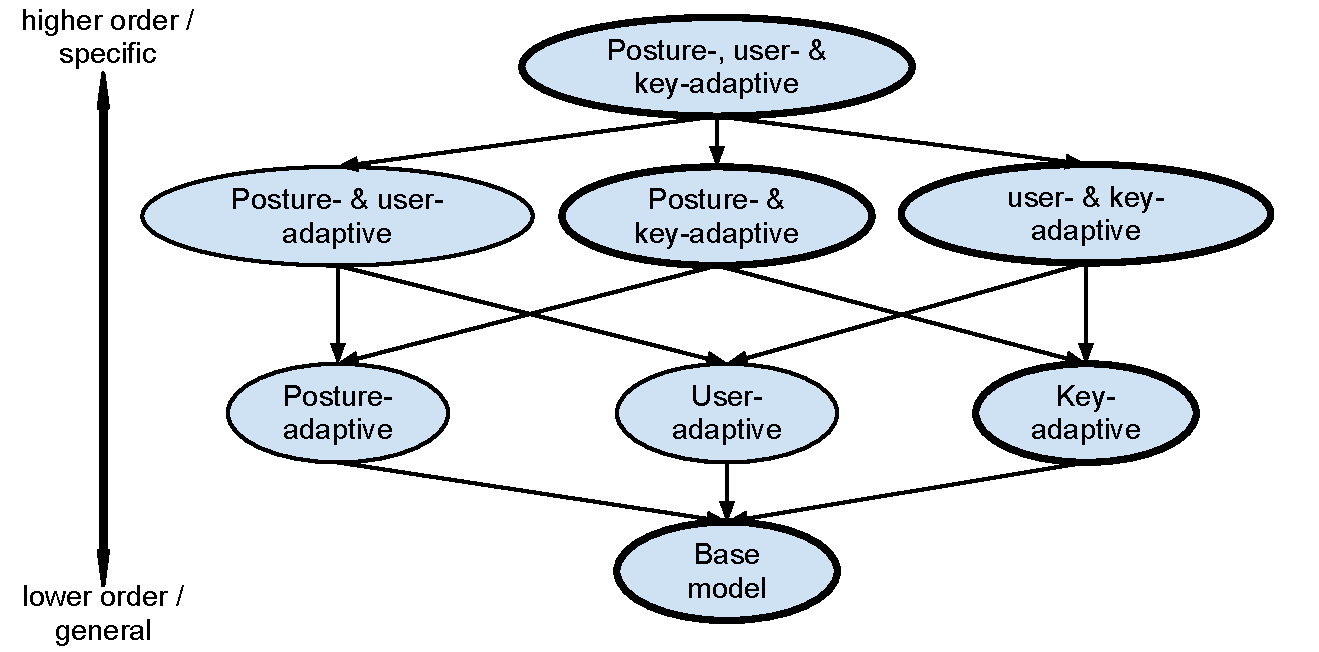
\includegraphics[width=0.9\columnwidth]{figures/hierarchy.pdf}
  \caption{A complete hierarchical spatial backoff model. For practical purposes, not all the submodels need to be included. The models with thicker lines are the ones we analyzed and included in the prototype implementation.}
  \label{fig:hierarchy}
\end{figure}

Each combination of the factors needs sufficient number of samples to build a reliable model. Hence, each submodel would only become \textit{mature} (active) when its reliability passes a set 
threshold. Otherwise a lower order model (backoff) will be used instead.

Figure~\ref{fig:hierarchy} shows a \textit{complete} hierarchy of the submodels with all
possible combinations of the three adaptive factors. However, depending on the
relative effectiveness of the submodels, it is not necessary to include all of
them in the implementation. In this paper, we focus on analyzing the key
adaptive model, posture and key adaptive model and user and key adaptive model.
The order of the
backoff process, and the priority of the models at the same level to use can
also be design choices, but the analysis in the next section gives
guidance and suggestion on how to determine the order.

\section{Key Estimation Formulation} 
As mentioned in the Research Methods section, our basic measure for analysis and comparison of the spatial models is character error rate. This is computed as
\begin{align}
\text{character error rate} = \frac{\text{No. wrongly estimated characters}}{\text{No. all target characters}}
\end{align}

Given $i$\textsuperscript{th} touch point coordinates $\underline c_i \in \mathbb{R}^2$, we estimate the input character as the most likely intended key, $\hat k_i$,  given by the following formulation:
\begin{align}
\hat k_i &= \arg\max_k p(k | \underline c_i; \underline \theta) \\
          &= \arg\max_k \frac{p(\underline c_i, k; \underline \theta)}{\sum_k p(\underline c_i, k; \underline \theta)} \\
          &= \arg\max_k p(\underline c_i, k; \underline \theta) \\
          &= \arg\max_k p(k;\underline\theta_l)p(\underline c_i | k; \underline \theta_s) \label{eq:likely-k}
\end{align}
where $\underline\theta_l$ represents the parameter vector of the language model and $\underline\theta_s$ represents the parameter vector of the spatial model. The $p(k;\underline\theta_l)$ term is related to the frequencies of letters and is part of the language model. To investigate the hypothesis that there is evidence in the data for adaptation of the spatial model, we analyze the effect in key estimation due to the spatial model alone as a first step. Hence we assume $p(k; \underline\theta_l)$ is the same for all $k$ (i.e. a uniform language model). As a result
\begin{align}
\hat k_i = \arg\max_k p(\underline c_i | k; \underline \theta_s)
\end{align}

The spatial model parameter vector $\underline \theta_s$ depends on the model selected from the hierarchical SBM. For example, when the posture, individual and key adaptive model is selected, then
\begin{align}          
\hat k_i = \arg\max_k \sum_{y, u} N(\underline c_i - \underline o_k; \underline\mu_{y,u,k}, \Sigma_{y,u,k})[[y = \textsf{y} \wedge u = \textsf{u}]]
\end{align}
where $\underline o_k$ is the center of the visual bounding box of key $k$, and $\underline c_i - \underline o_k$ 
represents the offset. $\textsf{y}$ and $\textsf{u}$ represent a particular value for the posture 
and the user respectively. $[[y = \textsf{y} \wedge u = \textsf{u}]] = 1$ if the 
statement is true, and $0$ otherwise. This is essentially making a hard decision on the 
posture and user variables for choosing the appropriate model parameters. For the user variable, 
this is reasonable because smartphones are personal devices and we can assume the 
same user typing on the same device. For the posture variable, potentially we could also 
use a soft decision and combine the probability distributions together based on the posture probability, $p(y)$. 

For the analysis in the Comparison of Spatial Models section, the values for $\textsf{y}$ and $\textsf{u}$ are 
\textit{observed} based on the dataset. This establishes the upper bound for the potential benefits from the adaptations. In section Implementation and Evaluation of the prototype, only the user is \textit{observed}; the value for the posture variable $\textsf{y}$ is \textit{inferred}.

\section{Comparison of Spatial Models}
We compare character error rate with different adaptive spatial models to analyze their
relative effectiveness (Table \ref{tab:comparison}). This can inform us the order of the
backoff models to use when there is not enough data for higher order models.
10-fold cross validation is used, and the training and testing data sets have different users.

\begin{table} [tb]
  \centering
  \begin{tabular}{|l|c|}
    \hline
    \tabhead{Spatial model} &
    \multicolumn{1}{|p{0.2\columnwidth}|}{\centering\tabhead{Character
    error rate}} \\
    \hline
    Distance from the center of the keys & 7.976\% \\
    \hline
    \multicolumn{1}{|p{0.7\columnwidth}|}{Base model (same Gaussian model $N(\underline 0, \Sigma)$ for
    all the keys with a full covariance matrix)} & 7.853\% \\
    \hline
    \multicolumn{1}{|p{0.7\columnwidth}|}{Key adaptive model, $N(\underline \mu_k, \Sigma_k)$} & 8.023\% \\
    \hline
    \multicolumn{1}{|p{0.7\columnwidth}|}{Posture \& key adaptive model, $N(\underline \mu_{y,k}, \Sigma_{y,k})$} & 7.058\% \\
    \hline
     \multicolumn{1}{|p{0.7\columnwidth}|}{Individual \& key adaptive model, $N(\underline \mu_{u,k}, \Sigma_{u,k})$} & 6.845\% \\
    \hline
  \end{tabular}
  \caption{Comparison of character error rate (no language model) with
  different spatial models using 10-fold cross validation. These results represent the theoretical upper bounds for the different adaptive spatial models based on our dataset since they assume \textit{observed} postures and intended keys for building the user specific models.}
  \label{tab:comparison}
\end{table}

The simplest model is a Gaussian distribution with zero mean $x$ and $y$
 offsets and the same spherical covariance matrix for all the keys. Key
detection based on this model is essentially choosing the key that has the shortest Euclidean distance from the tapping coordinates. 
Our base model has a full covariance matrix $\Sigma$ trained from the
training data, but the same base model $N(\underline 0, \Sigma)$ is used for all keys. Hence, when using the base model for key estimation, the most likely intended key is
\begin{align}          
\hat k = \arg\max_k N(\underline c_i - \underline o_k; \underline 0, \Sigma)
\end{align}


\subsection{Key Adaptation}
A basic key adaptive model has one bivariate Gaussian model
$N(\underline\mu_k, \Sigma_k)$ for each key $k$ built  using data from all users in the training dataset. The most likely intended key based on key adaptive model is
\begin{align}          
\hat k_i = \arg\max_k N(\underline c_i - \underline o_k; \underline \mu_k, \Sigma_k)
\end{align}

The result in Table~\ref{tab:comparison} shows no improvement of key adaptive model over the base model. This is because different hand postures tend to shift key specific spatial model in different ways, sometimes even in opposite directions. For example in Figure \ref{fig:key-adaptive}, we observe that the effective area of W key goes slightly beyond the visual key boundary between E and W. For one-finger input, there tend to right horizontal offsets for W key, while for two-thumb input, there tend to be left horizontal offsets. When mixing these opposite effects together in key adaptation, no meaningful results could be expected.

\begin{figure}[tb]
  \centering
  \subfigure[Key adaptive model]{
    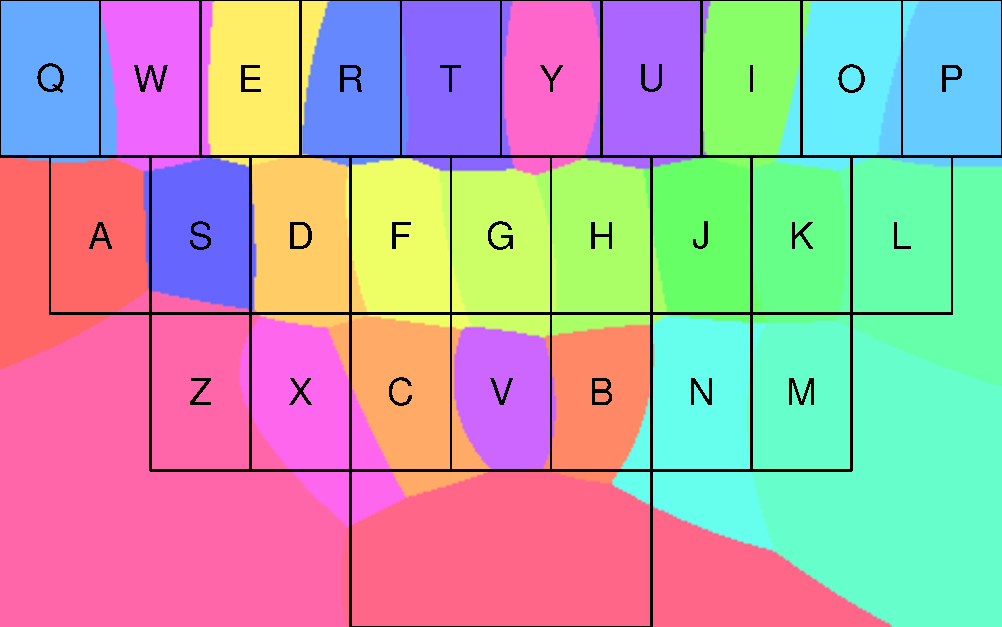
\includegraphics[width=0.47\columnwidth]{figures/key-model.pdf}
    \label{fig:key-adaptive}
  } ~
  \subfigure[Posture and key adaptive model for one-finger input]{
    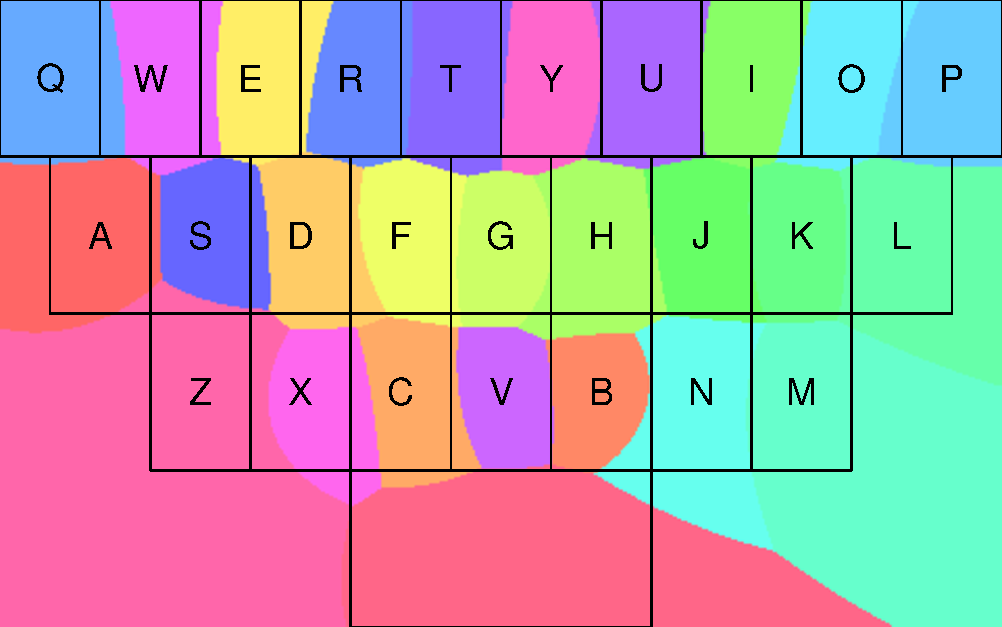
\includegraphics[width=0.47\columnwidth]{figures/posture-t.pdf}
    \label{fig:one-finger}
  }
  \subfigure[Posture and key adaptive model for two-thumb input]{
    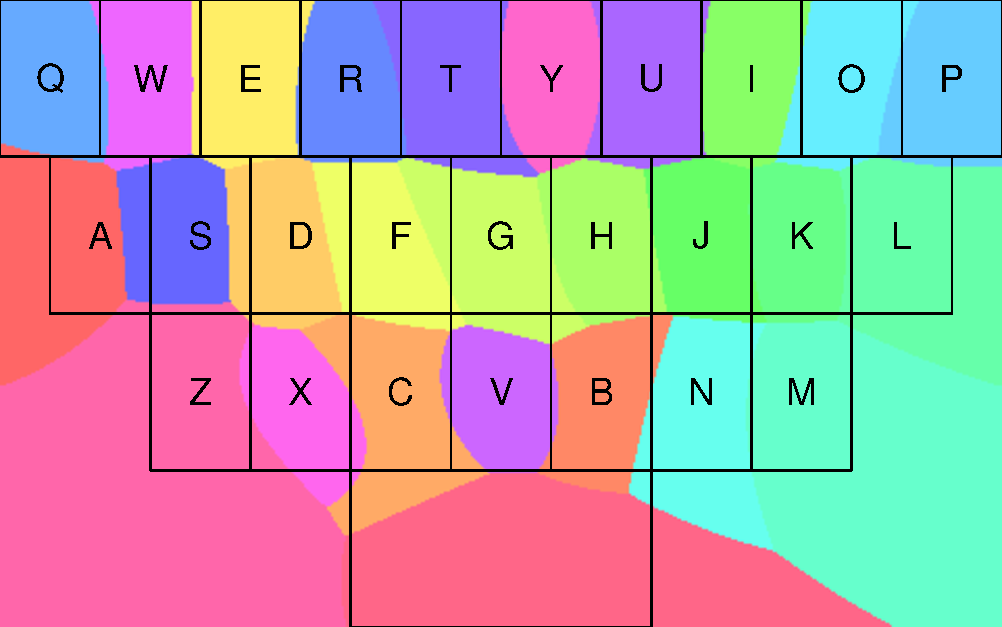
\includegraphics[width=0.47\columnwidth]{figures/posture-tt.pdf}
    \label{fig:two-thumb}
  }
  \caption{Comparison of effective key areas with different spatial models.  Each colored area presents the region such that if the user taps in that region, the spatial model will classify that key with the corresponding key label.}
  \label{fig:key-boundary}
\end{figure}

\subsection{Posture Adaptation}
Key adaptation becomes more effective when combined with posture adaptation as
shown in Table~\ref{tab:comparison}. There is 12.0\% reduction in error rate 
compared to key adaptation only. The two-sample one-sided paired t-test shows
that the improvement in accuracy is significant when we use posture and key 
adaptation versus key adaptation only (t(29) = -2.4421, p = 0.01).

There can be different levels of complexity for posture adaptation. For the most complex one, we can have
two models for each key for each input posture, i.e., $N(\underline \mu_{y,k}, \Sigma_{y,k})$ for $y \in
\{\text{one-finger, two-thumb}\}$; or we can do posture adaptation only for a certain
number of keys. The best result is obtained when we only do posture adaptation for the keys on 
the left side, and for the keys on the right side, their Gaussian models are
independent of the posture, i.e., $N(\underline\mu_k, \Sigma_k)$.
The error rate for posture and key adaption shown in Table~\ref{tab:comparison} is based on 
posture adaptation for the keys on the left side. This approach is similar to the ``parameter tying'' technique that is often used in acoustic modeling in speech recognition~\cite{Bellegarda:1989} and natural language processing~\cite{Lin:1995} to deal with insufficient training data.

From (\ref{eq:likely-k}), the most likely intended key based on posture and key adaptive model can be written as
\begin{align}          
\hat k_i = \arg\max_k \sum_{y} p(\underline c_i | k, y; \underline\theta_s)[[y = \textsf{y}]],
\end{align}
where
\begin{align}
p(\underline c_i | k, y; \underline\theta_s) = \left\{
  \begin{array}{l l}
  N(\underline c_i - \underline o_k; \underline \mu_{y, k}, \Sigma_{y,k}) & \text{if $k$ is on left side} \\
  N(\underline c_i - \underline o_k; \underline \mu_{k}, \Sigma_{k}) & \text{if $k$ is on right side} \\
\end{array} \right.
\end{align}

The choice of this set of keys is not arbitrary. As observed by Azenkot et al. \cite{Azenkot:2012}, the difference in horizontal
offsets of the touch points from different postures are most prominent for the keys on the
left side (Note that for left-handed users, the reverse is probably true). 
In addition, the analysis of variance based on the tapping coordinates from the
dataset shows that, for different postures, there are significant differences in the means of
the $x$ coordinate for the keys on the left side of the keyboard ($p < 0.05$). 

Figure~\ref{fig:one-finger} and \ref{fig:two-thumb} show the comparison of effective areas of the keys
with spatial models adapted to one-finger input and two-thumb input respectively. Note how the key areas for the left-side keys shift to the left
for two-thumb input, and shift to the right for one-finger input. The difference in 
the effective key areas is the same concept as key-target resizing mentioned in \cite{Gunawardana:2010, Rudchenko:2011}.

The error rate in Table~\ref{tab:comparison} is based on perfect knowledge of
the posture. In the real-world implementation, the online posture classification may
introduce errors. To mitigate the problem, the posture adaptive model can be turned on
when the posture classification confidence is high. The details are explained in a later section.

\subsection{Individual Adaptation}
The individual and key adaptive model gives a 14.7\% error reduction over key adaptive model. As some data is needed to build the individual and key specific model, the most likely intended key $\hat k_i$ can be written as
\begin{align}          
\hat k_i = \arg\max_k \sum_{u} p(\underline c_i | k, u; \underline\theta_s)[[u = \textsf{u}]],
\end{align}
where
\begin{align}
p(\underline c_i | k, u; \underline\theta_s) = \left\{
  \begin{array}{l l}
  N(\underline c_i - \underline o_k; \underline \mu_{k}, \Sigma_{k}) & \text{if $i \le T_\text{user}$} \\
  N(\underline c_i -  \underline o_k; \underline \mu_{u, k}, \Sigma_{u, k}) & \text{if $i >T_\text{user}$} \\
\end{array} \right. \label{eq:user-adaptive}
\end{align}
$T_\text{user}$ is the minimum number of data points needed to build a user specific key model. 
It can be key dependent, i.e. $T_\text{user, k}$ for each key $k$, or not. Equation~(\ref{eq:user-adaptive}) 
essentially shows the backoff mechanism for the user and key adaptive model.

The result in the last row of Table~\ref{tab:comparison} is based on the 
following method. For each fold of the cross-validation, data from the training set are used to 
train the combined backoff key models. For each user $u$ in the test set,
50\% of the data for each key is used to train the individual and key adaptive
model, i.e., $N(\underline \mu_{u, k}, \Sigma_{u, k})$.
The accuracy of these data points are tested on the combined key models.
The remaining 50\% of the data for each user are tested on the user and key adaptive 
model. 

Figure~\ref{fig:user-adapt} shows how key estimation error rate for key E 
changes as the number of points used to build
the personalized model for key E increases. The error rates are obtained using cross-validation
and are based on the touch points that are not used in building the
model. We choose E as an
example because it has the most number of data points (around 90) for each
user in our dataset besides the ``Space'' key. It is hard to do the analysis for the other keys with
relatively small number of data points. However, we believe the result would be applicable to other
keys. Also due to the limited number
of data points, we only show the trend until the number of touch points used to build the individual
model is 70. Nevertheless, the figure still shows a general trend, and suggests 
that the minimum number of data points for building a individual key adaptive model
should be at least 60, but a number in the order of a hundred is probably better. 

\begin{figure}[tb]
  \centering
  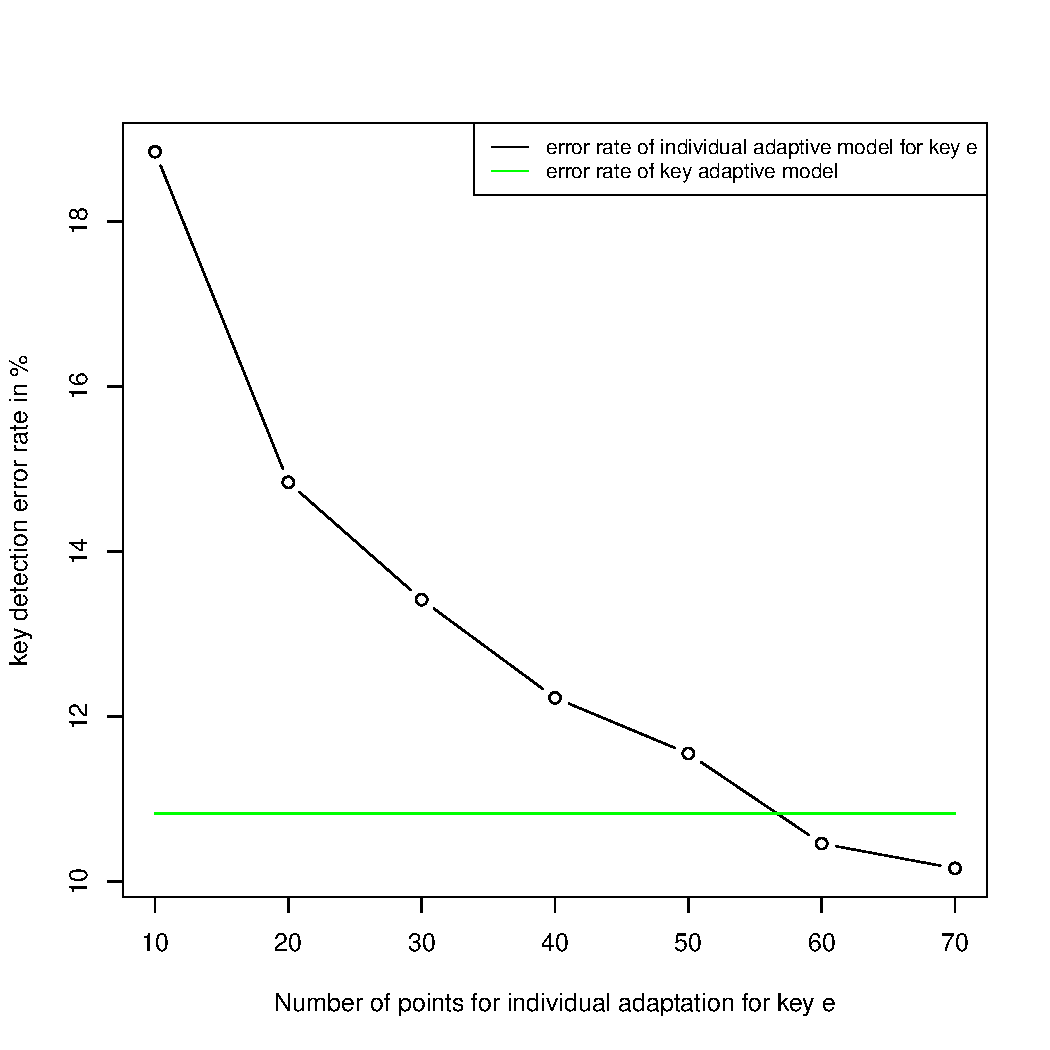
\includegraphics[width=0.9\columnwidth]{figures/individual-adapt.pdf}
  \caption{Graph showing how key estimation error rate for key E changes as the number of
  points used to build the individual adaptive model for key E increases.}
  \label{fig:user-adapt}
\end{figure}

\section{Input Hand Posture Classification}\label{sec:posture-classification}
The hierarchical adaptive SBM needs real time classification of the user's hand postures. 
A variety of sensors, signals and algorithms can be used in the future to achieve such a
 function. We developed an online binary hand-posture classifier 
that constantly returns an estimate of the user's current posture  $y \in \{\text{two-thumb, one-finger}\}$ from the 
user's input touch points without additional sensors. 

Our method is based on Fitts' law which states that the time ($T$) required to move to a target is a function of the distance ($D$) to the target and the size ($W$) of the target:
\begin{align}
T = a + b\log_2(1 + \frac{D}{W})
\end{align}                                                  
We expect one-finger input posture follows this law,  but two-thumb input may not. For example, a user may take a longer time to type the letters AL using one finger because the finger has to travel a longer distance from key A to key L on a Qwerty keyboard. With two thumbs, typing AL can be faster because the touch action switches from left thumb to type A to the right thumb to type L, and no long distance travel is required.

\begin{figure}[tb]
  \centering
  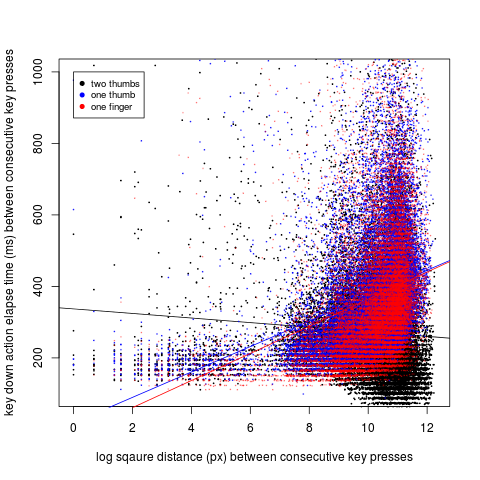
\includegraphics[width=0.9\columnwidth]{figures/time-distance.png}
  \caption{Touch points data from input on a Nexus S phone.}
  \label{fig:time-distance}
\end{figure}

Figure. \ref{fig:time-distance} shows the relationship between the time elapsed 
and the log square distance travelled between consecutive key taps. For the one-finger input (blue and red points), the time taken
increases with distance whereas for the two-thumb input, there is no obvious
trend. The difference is more significant when the log square distance (natural
log) is greater than 10 px.

Based on this finding, we include the time elapsed and the log square distance
between two consecutive key presses as the features for the posture classifier. 
To account for individual typing speed differences, we also use normalized time 
elapsed between consecutive key presses as the third feature. It is calculated 
by dividing the time elapsed by the average time elapsed for the last 10 key
taps.

Using 20 users’ data for training and 10 users’ data for testing, we train a SVM classifier offline with these 3 features for touch points that satisfy condition $C$: it is 
on the different side of the keyboard from its previous touch point and the log square distance from the previous touch point is at least 10px. This classifier gives a probability score $p_y^{\text{single}}$ for these touch points. Note that $\displaystyle\sum_{y \in \mathcal{Y}}p_y^{\text{single}} = 1$. The posture classification accuracy for these touch points is 83.6\%.
 
In order to classify every key tap and assuming the user does not change posture 
rapidly, we look at a sliding time window of 10 touch points (about 2 words). For 
each time window, we use another SVM classifier with the following features:
\begin{enumerate}
\item Correlation between time elapsed and log distance (this feature has the
advantage of being speed independent) (see Figure. \ref{fig:boxplot}).
\item Sum of $p_\text{one-finger}^{\text{single}}$ for touch points satisfying condition $C$.
\item Sum $p_\text{two-thumb}^{\text{single}}$ for touch points satisfying condition $C$.
\item Number of touch points classified as one-finger input.
\item Number of touch points classified as two-thumb input.
\end{enumerate}
Features 2-4 are also normalized by the window size. The history of the touch points are cleared for every new typing session.
The choice of the size of the sliding window represents a trade-off between the 
accuracy of the classification and how responsive the system is when the user
changes posture. We found that the assumption that the user does not change posture
often within 2 words is reasonable, but more work can be done to investigate this
aspect, and even to test with a window size of 1 (i.e. not 
looking at the history).

The sliding time window classifier gives a final probability score $p_y$ for posture
$y$ for each touch point. Again $\displaystyle\sum_{y\in \mathcal{Y}}p_y = 1$. To evaluate the classification accuracy, we set the the
classified posture to be $y$ if $p_y > 0.5$. With this, the overall classification 
accuracy for each touch point with a sliding time window
is 86.4\% (23128 out of 26769 touch points).

Because of the sliding window approach, the posture for the first few touch points  
for each new session is unknown. In this case, the system backed off to a lower order spatial 
model (key adaptive or base model). Furthermore  it turns on the posture 
adaptive spatial model only when the probability score for one posture is much 
higher than the other.

\begin{figure}[tb]
  \centering
  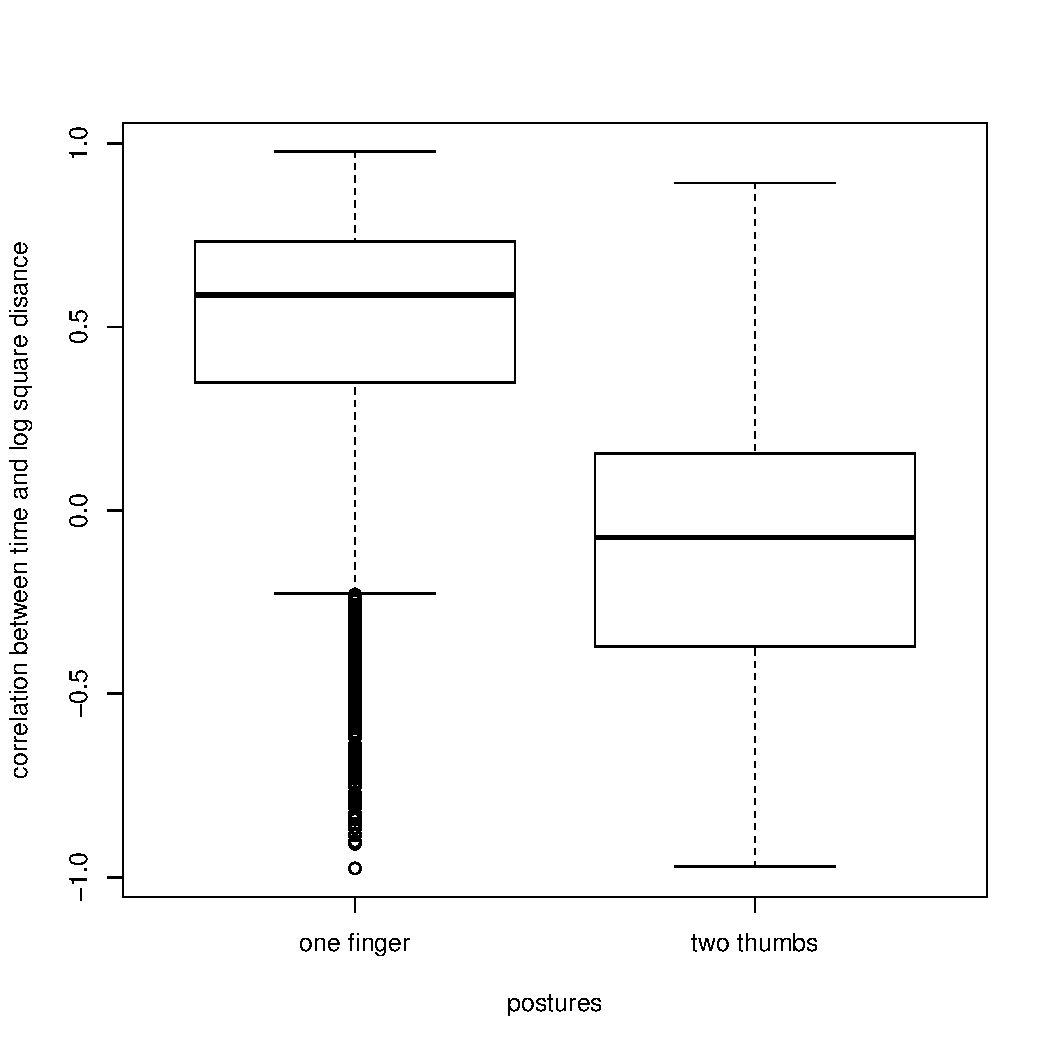
\includegraphics[width=0.8\columnwidth]{figures/boxplot.pdf}
  \caption{Correlation between time elapsed and log square distance between
  consecutive key presses for every 10 keys. There is a stronger correlation for
  one- finger input than that for two-thumb input.}
  \label{fig:boxplot}
\end{figure}

\section{Implementation and Evaluation}
The key estimation process with the proposed SBM fits nicely with the
Chain of Responsibility design pattern.
Figure~\ref{fig:chain-of-responsibility} shows a simplified version of an object
diagram showing the interaction between various models. Each higher order model can
have a reference or references to lower order models. When given a pair of touch
point coordinates, the system queries the highest order model for a Gaussian
submodel for a particular individual/posture/key combination. If it is not present, 
the higher model calls the lower model, and the
query propagates until a Gaussian sub-model is found. 

\begin{figure}[tb]
  \centering
  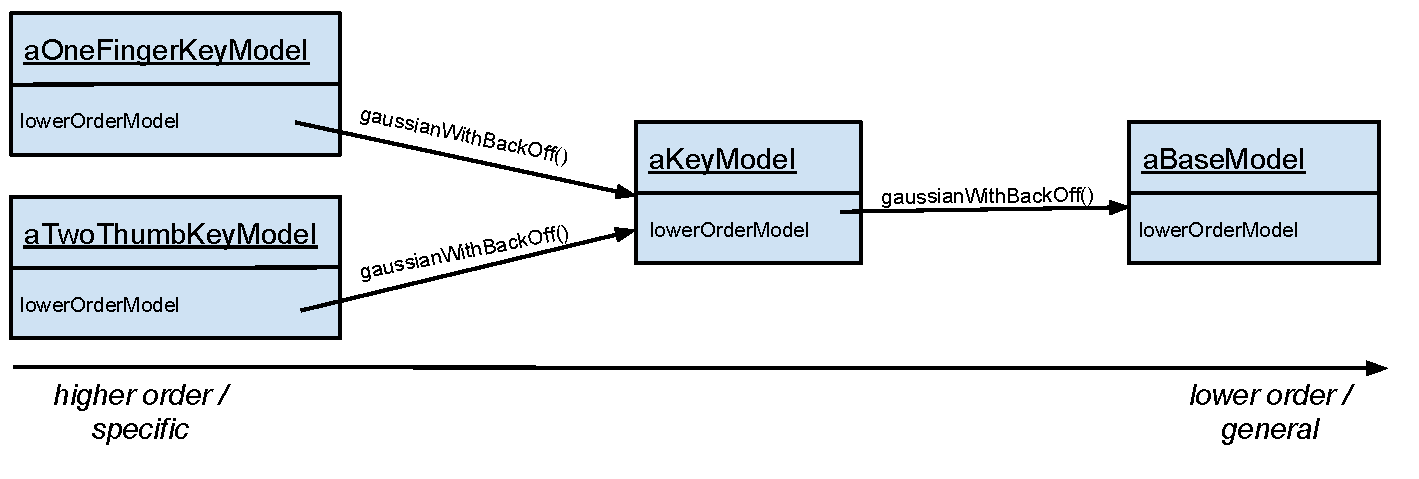
\includegraphics[width=1\columnwidth]{figures/chain-of-responsibility.pdf}
  \caption{An object diagram showing the interaction between higher and lower
  order spatial models.}
  \label{fig:chain-of-responsibility}
\end{figure}

Based on this design, we implemented a prototype of SBM with the online posture 
classification in C++. The prototype SBM has flags to turn on/off certain adaptive
 models so that we can easily compare the effectiveness of submodels in this real-world implementation. 
 For all the evaluations, we use 20 users' data for training both the posture classifier 
 and the spatial models, and the other 10 users' data for testing. 

\subsection{Evaluation of Standalone SBM}
Like \cite{Findlater:2012, Rudchenko:2011}, we evaluate the effectiveness of the standalone SBM  prototype on key estimation without a language model first. 
Table~\ref{tab:off-device} shows the comparison of
character error rates using SBM with different submodels turned on. The main difference between these results and those in Table~\ref{tab:comparison} is that in the prototype implementation posture is \textit{inferred} and the user specific model is built according to \textit{inferred} intended key.

\begin{table}[tb]
  \centering
  \begin{tabular}{|l|c|}
  \hline
  \tabhead{Highest order spatial model in SBM} &   \multicolumn{1}{|p{0.2\columnwidth}|}{\tabhead{Character error rate}} \\
  \hline
 Base model & 8.641\% \\
  \hline
  Key adaptive model & 8.708\% \\
  \hline
    \multicolumn{1}{|p{0.7\columnwidth}|}{Posture and key adaptive model} & 8.394\% \\
  \hline
  Individual and key adaptive model  & 7.621\%
  \\
  \hline
  Posture, individual and key adaptive model &  7.498\%
  \\
  \hline
  \end{tabular}
  \caption{Comparison of character error rates using the real-world implementation of the standalone SBM model with different submodels turned on.  These results are based on \textit{inferred} postures and intended keys for building the user specific models. Results are based on 10 test users.}
  \label{tab:off-device}
\end{table}

\subsubsection{Posture Adaptation}\label{sec:off-device-posture}
The posture and key adaptive model uses the posture classification
method described in the previous section. As a result, the
key detection error rate for using this model is compounded with the posture
classification error rate as well. 

An error in posture classification will lead to a choice of wrong submodel,
and hence adversely affect the key detection accuracy. The confidence of the classification is reflected by the pair of probability 
scores $(p_{\text{one-finger}}, p_{\text{two-thumb}})$ returned by the classifier. 
We can set a threshold $T_{\text{posture}}$ such that the input posture is classified
as $\textsf{y}$ only if $P_\textsf{y} \ge T_{\text{posture}}$ . Otherwise the posture is treated as
unknown and we backoff to a lower order spatial model.

There is also a trade-off in setting the threshold $T_{\text{posture}}$. The higher
 $T_{\text{posture}}$ is, the fewer the number of errors there are in posture classification, but it also means the more touch points will be classified as from unknown posture and no posture adaptation is used for these touch points. Figure~\ref{fig:posture-confidence} 
 shows that there is an optimal level of the threshold beyond which the error rate
 increases because we no longer take the advantage of posture adaptation. The error rate in Table~\ref{tab:off-device} for SBM with posture and key adaptive model as the highest order model is obtained by setting $T_{\text{posture}} = 0.94$.

\begin{figure}[tb]
 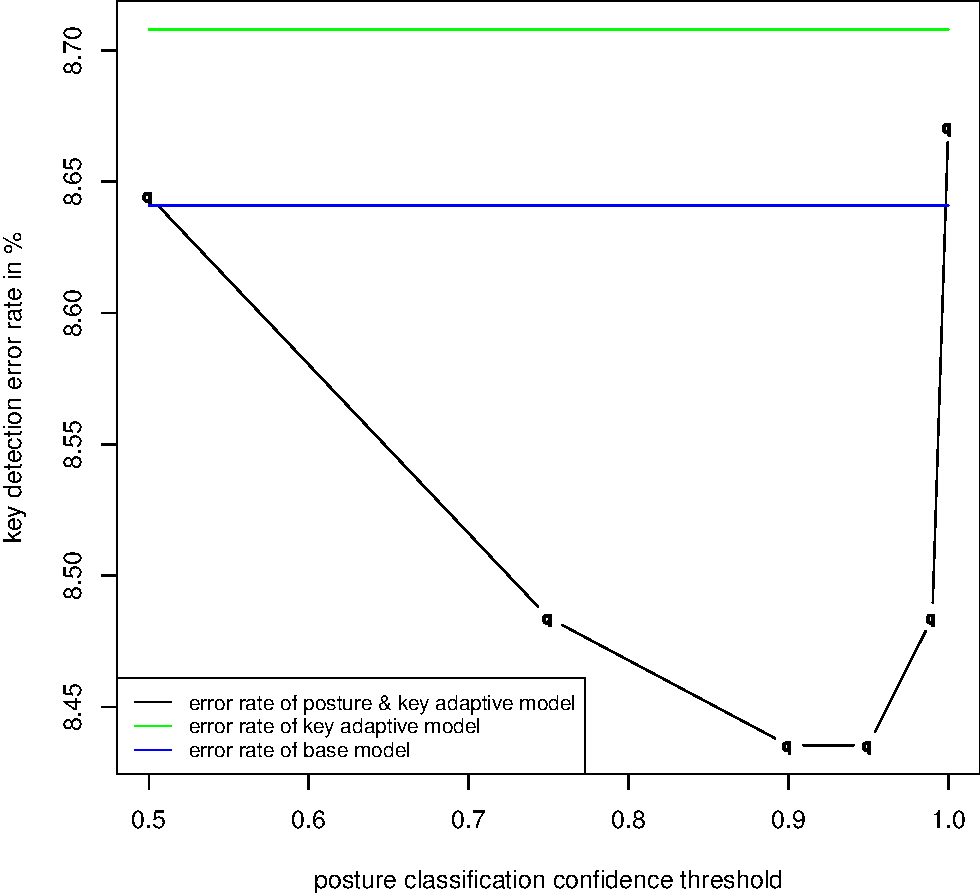
\includegraphics[width=0.9\columnwidth]{figures/error-confidence-cropped.pdf}
  \caption{Graph showing how key estimation error rate changes as the confidence
  threshold for posture classification increases.}
  \label{fig:posture-confidence}
\end{figure}

To further investigate the effect of posture adaptation, we look at the key estimation
errors represented in confusion matrices (see Figure~\ref{fig:confusion-matrices}). Figure~\ref{fig:error-key} and \ref{fig:error-posture}
show the errors when using key adaptive model, and posture and key adaptive model respectively. Figure~\ref{fig:error-key-posture}
and \ref{fig:error-posture-key} shows errors in one model but not the other.
We can see that when using posture and key adaptive model we also incur errors
that are not present when using key adaptive model alone. However the number of these
errors are much smaller compared to the errors corrected.

\begin{figure*}[tb]
  \centering
  \subfigure[Errors when using key adaptive model]{
    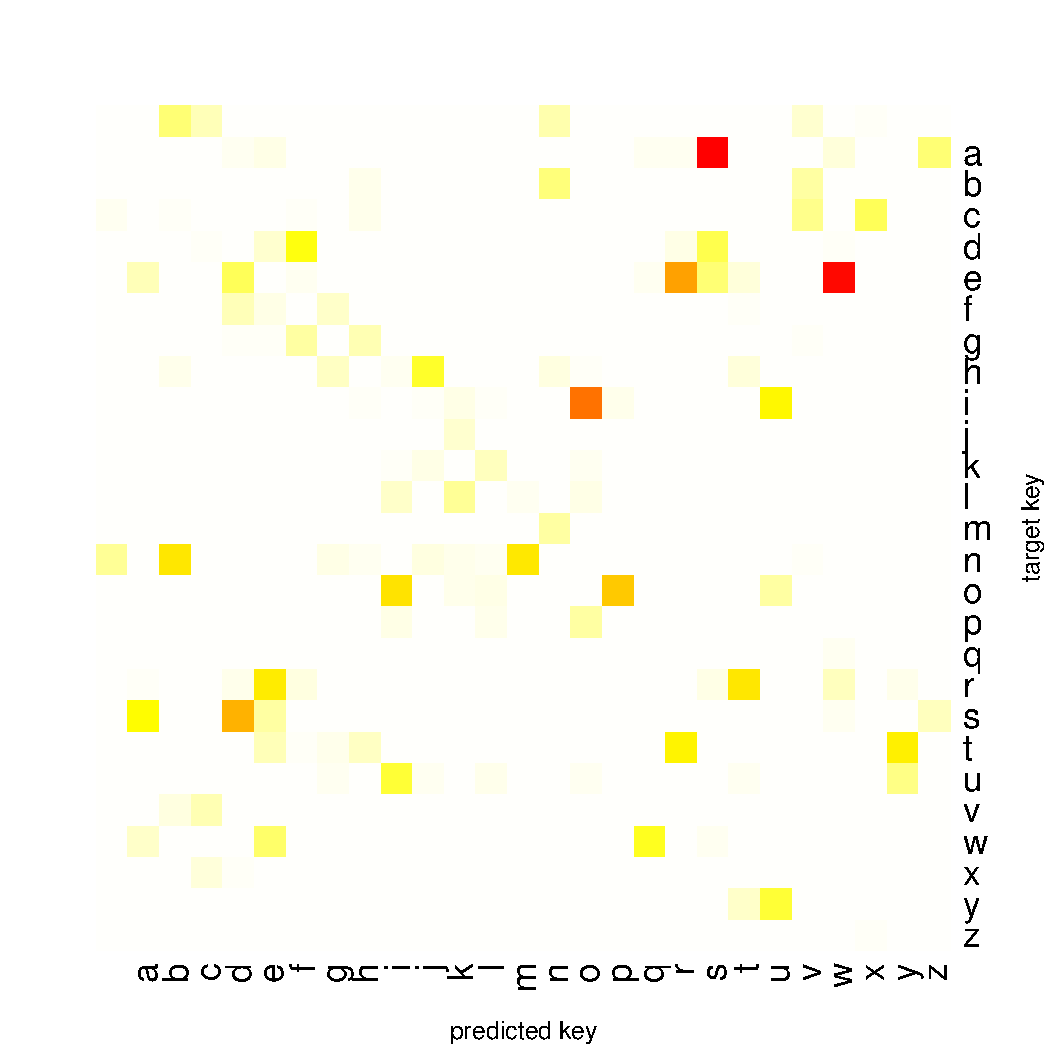
\includegraphics[width=0.49\columnwidth]{figures/sim-result-1.pdf}
    \label{fig:error-key}
  } 
  \subfigure[Errors when using posture and key adaptive model]{
    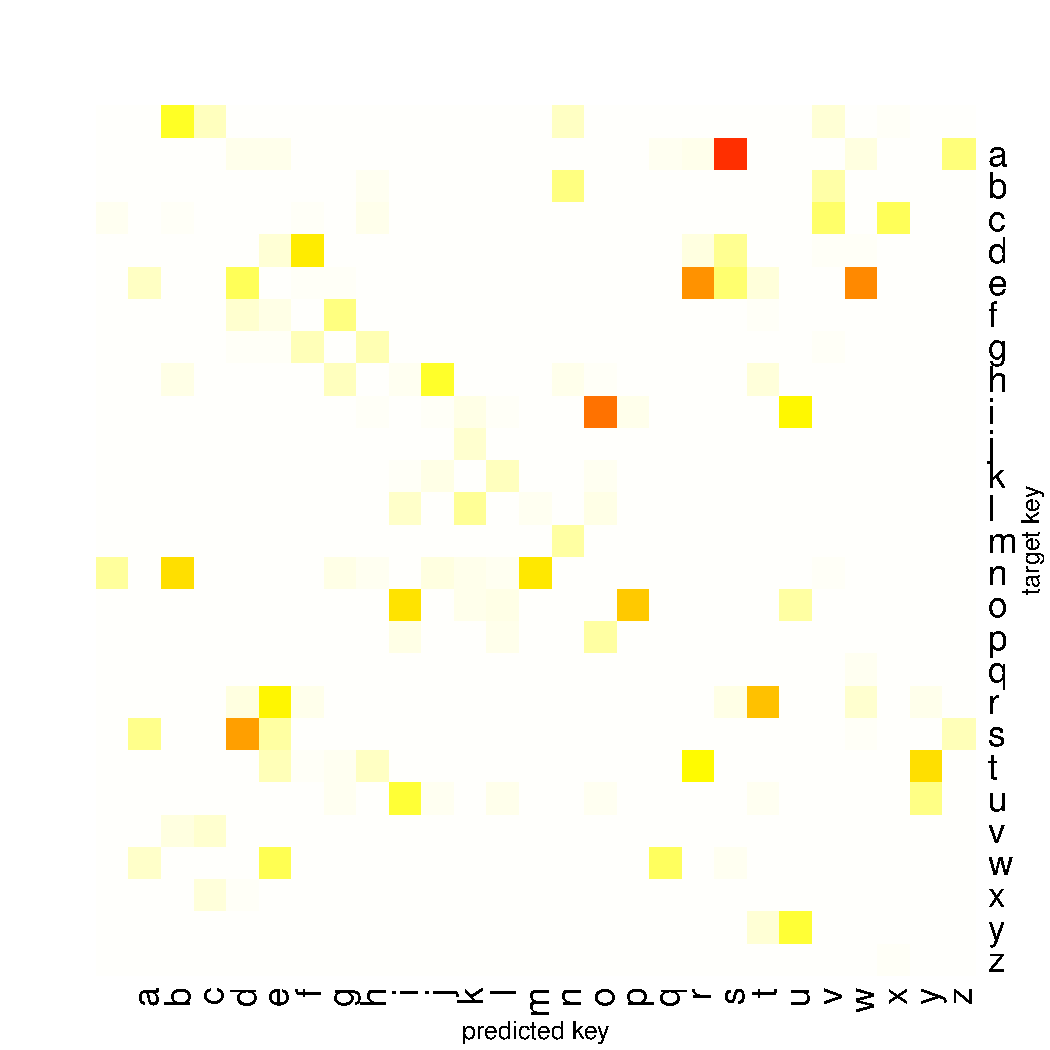
\includegraphics[width=0.49\columnwidth]{figures/sim-result-2.pdf}
    \label{fig:error-posture}
  }
  \subfigure[Errors when using key adaptive model but not when using posture and key
  adaptive model]{
    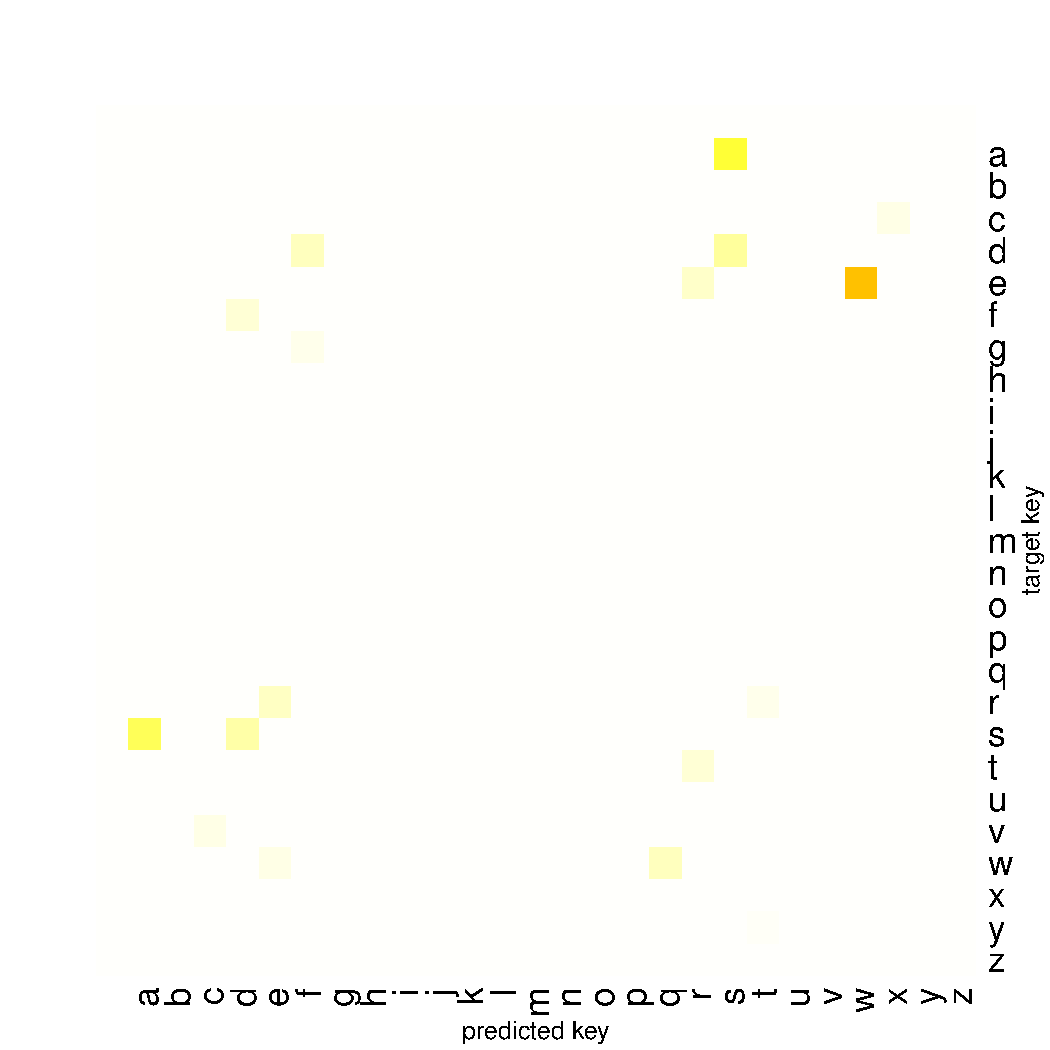
\includegraphics[width=0.49\columnwidth]{figures/sim-result-1-2.pdf}
    \label{fig:error-key-posture}
  }
  \subfigure[Errors when using posture and key adaptive model but not when using key
  adaptive model]{
    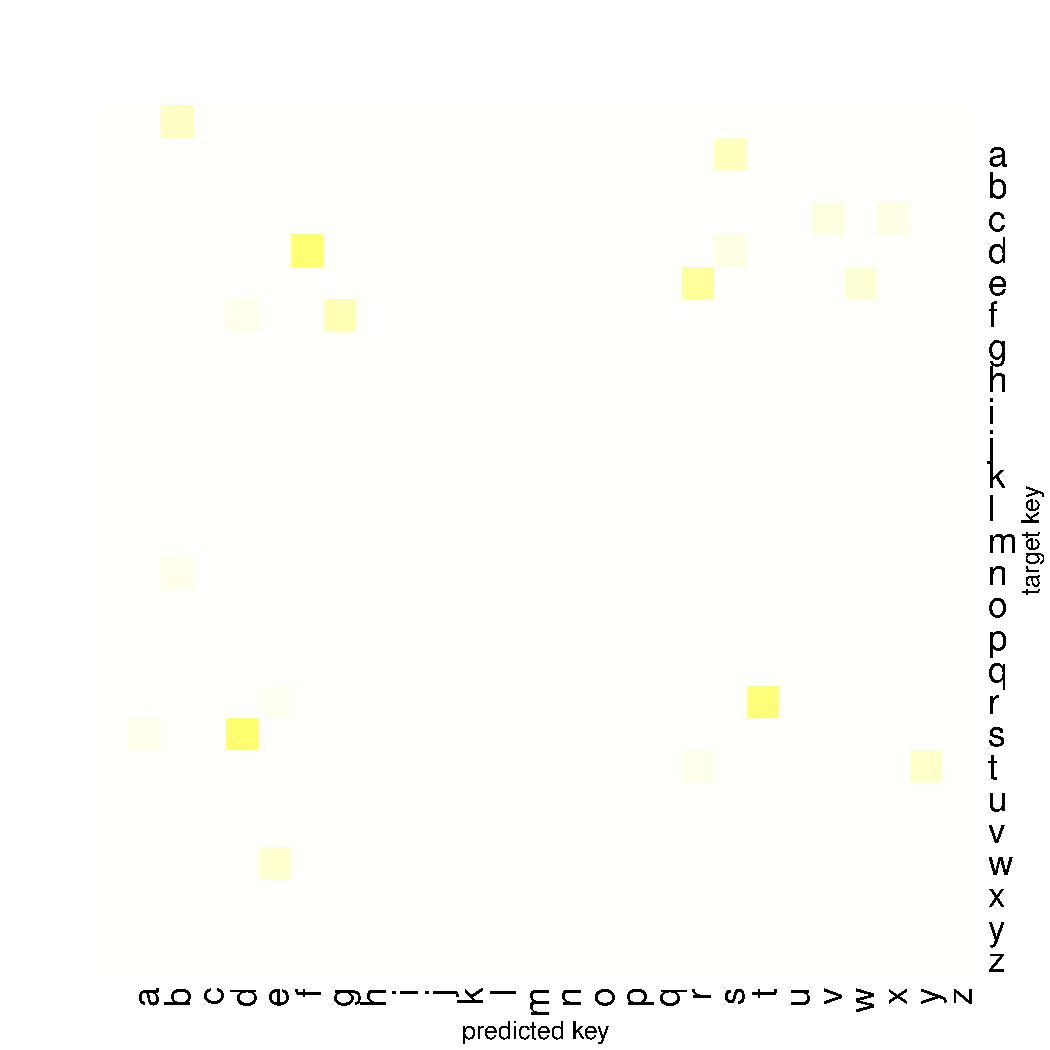
\includegraphics[width=0.49\columnwidth]{figures/sim-result-2-1.pdf}
    \label{fig:error-posture-key}
  }
  \subfigure{
    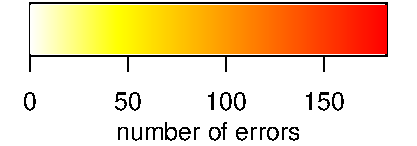
\includegraphics[width=0.3\columnwidth]{figures/sim-result-colorkey.pdf}
  }
  \caption{Confusion matrices for key estimation evaluation with different
  spatial models as the highest order model. The row labels are the
  target keys, and the column labels are the predicted keys.  The color of the cells
represents the number of errors for a particular pair of confusion. The more red the color,
the greater the number of errors.}
  \label{fig:confusion-matrices}
\end{figure*}

Figure~\ref{fig:error-key-posture} also shows that the most number of
corrections by using posture and key adaptive model is for the E and W pair. Figure~\ref{fig:e-w-ellipses}
shows a closer look at the Gaussian distributions for the two keys for the different
adaptive models. We can see the Gaussian distributions for key adaptive model (black ellipses) shift slightly to the right. This causes the touch points on the boundary between W and 
E to be mis-classified as W. However, the ellipses based on the posture and key
adaptive model for the two-thumb input shift to the left slightly, and this changes
the classification of those boundary points to E correctly.

\begin{figure}[tb]
  \centering
  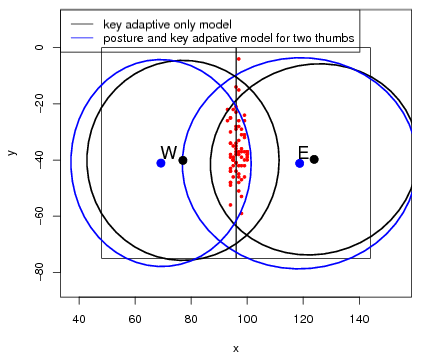
\includegraphics[width=1\columnwidth]{figures/key-posture-ellipse.png}
  \caption{Each ellipse represents the 0.95 confidence ellipse of the Gaussian model built based on a set of touch points. Each black ellipse is based on the all touch points intended for either W or E. Each blue ellipse is based on touch points from two-thumb input only. The red points are the touch points intended for E but are mis-classified as W when using the key adaptive model. 
}
  \label{fig:e-w-ellipses}
\end{figure}

\subsubsection{Individual Adaptation}
For the individual and key adaptive model, we set the minimum number of points needed to build the
Gaussian model for a particular key for a particular individual to be 50. Ideally we would want like to set this number higher for better model reliability as shown in Figure~\ref{fig:user-adapt}. However the current number is 
limited by the amount of data we have because there are not many keys that has 
the number of touch points be greater than 50 in our dataset. 

For every touch point, we compute the probability for each key given the underlying spatial model. Then we use the $(x, y)$ coordinates of the touch point to update the Gaussian model
for the most probable key. Updating the Gaussian model involves computing the running
average of the $(x, y)$ offsets from the center of the key and the covariance matrices. The counter for the number of points used for a particular key Gaussian is maintained so that we
know when a particular Gaussian model is \textit{mature}. When there is not enough data points, the system backs-off to a lower order model.

\subsubsection{Posture, Individual and Key Adaptation}
Tying everything together, the last row in Table~\ref{tab:off-device} shows the error rate when the highest order model is posture, individual and key adaptive. It gives an error reduction of about 13.2\% compared to the base model.

Figure~\ref{fig:partial-hierarchy} shows the backoff mechanism when there is insufficient data for the highest order model. The results based on our dataset in the Comparison of Spatial Models section suggest that we
can give higher priority to individual and key adaptive model when we do not have enough data for
the highest order model. If there are still not enough data for that, we 
can backoff to posture and key adaptive model. 

\begin{figure}
  \centering
  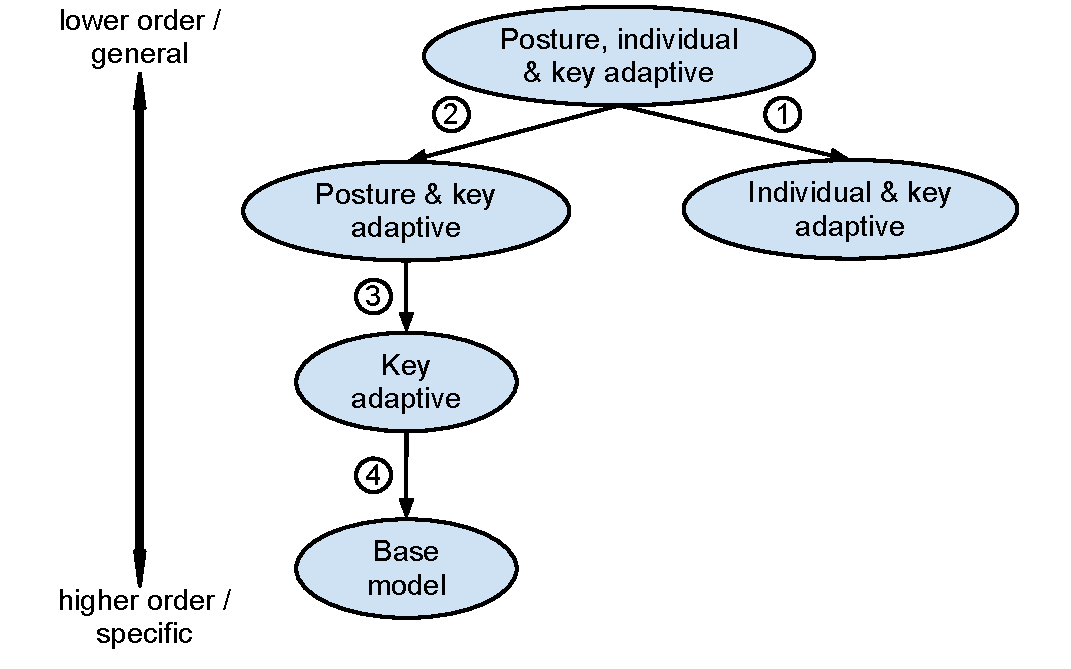
\includegraphics[width=0.9\columnwidth]{figures/partial-hierarchy.pdf}
  \caption{Partial hierarchical model implemented in our prototype. The numbers indicate the order of the 
submodels to use during backoff.}
  \label{fig:partial-hierarchy}
\end{figure}
Note that because the dataset is based on a between-user study, we cannot look
at the full effect of posture adaptation for each individual. We hypothesize that there could potentially be more improvement, but further study is required to verify this.

\section{Discussion}
We have shown the potential of posture, individual and key adaptation in improving key estimation by considering the spatial model alone. 
More work is needed to explore the interaction between spatial adaptation and
language modeling. It would also be interesting to study how
to use posture detection to guide transposition error correction, because transposition error
is more likely to occur when two hands are used to type.

An important limitation of our exploration thus far is the limited dataset available. To advance this line of work further we would ideally need greater amounts of data than what is typically collectable from lab experiments. Methods such as real use logging with strict privacy preservation and game playing~\cite{Rudchenko:2011} can be possibly employed to gather a large body of data. Because of the dataset limit, what we have addressed is fundamentally an \textit{approach} to STK spatial model adaptation. The specific (sub)models, the backoff procedure and sequence, and certainly the parameters learned from the data, may be changed and optimized in the future. 

\section{Conclusion}
We have introduced and evaluated a novel hierarchical adaptive spatial model for
touchscreen keyboard. Through comparative submodel analysis,  evaluation of a prototype implementation, we have shown that both posture and user adaptation for the spatial model can improve key estimation accuracy. When posture, individual and key adaptations are combined, they can
give the most improvement. For real-world
implementation, the
hierarchical structure gives a systematic way of backing-off to successively simpler models  when data is limited
or when there is not sufficient confidence for higher level models (e.g., when the posture classification confidence is not 
high enough).

We have also developed a new touchscreen input posture classification method
that achieves an accuracy of 86.4\% for classifying one-finger and two-thumb input. When
combined with the adaptive spatial model, the overall key detection accuracy is increased
in our simulation.
\section{Acknowledgments}
We want to thank our team members (names omitted for review) for their insightful
suggestions and help in  our data analysis and implementation of the prototype.
\balance
% If you want to use smaller typesetting for the reference list,
% uncomment the following line:
\small
\bibliographystyle{acm-sigchi}
\bibliography{chi2013}
\end{document}

